\chapter{Related Work}
\begin{quote}
\emph{This chapter summarizes research in citizen science, lead-user innovation, and social computing that inform the design of systems in this dissertation. Citizen scientists have successfully solved expert-defined problems as sensors or algorithms. However, public involvement in scientific endeavors fail to provide a true participatory experience that is citizen-led and personally meaningful. Lead-user innovation provides a complementary setup. Lived experience, a tight feedback loop, and strong personal motivation enable people to create different and sometimes better products than experts; however, lead users rarely have access to training, conceptual knowledge, and pre-existing organizational structure for collaboration. Finally, social computing and crowdsourcing platforms support sharing potentially novel ideas but converting these to actionable plans requires expert guidance. This dissertation provides ways to integrate learning in social computing to enable deeper contributions from citizen scientists and lead users without expert involvement.} 
\end{quote}

%Professionals have the advantages of training, conceptual knowledge, and pre-existing organizational structure for collaboration and support; however, lead users rarely have access to such systematic support.

\begin{figure}[h] 
  \centering
  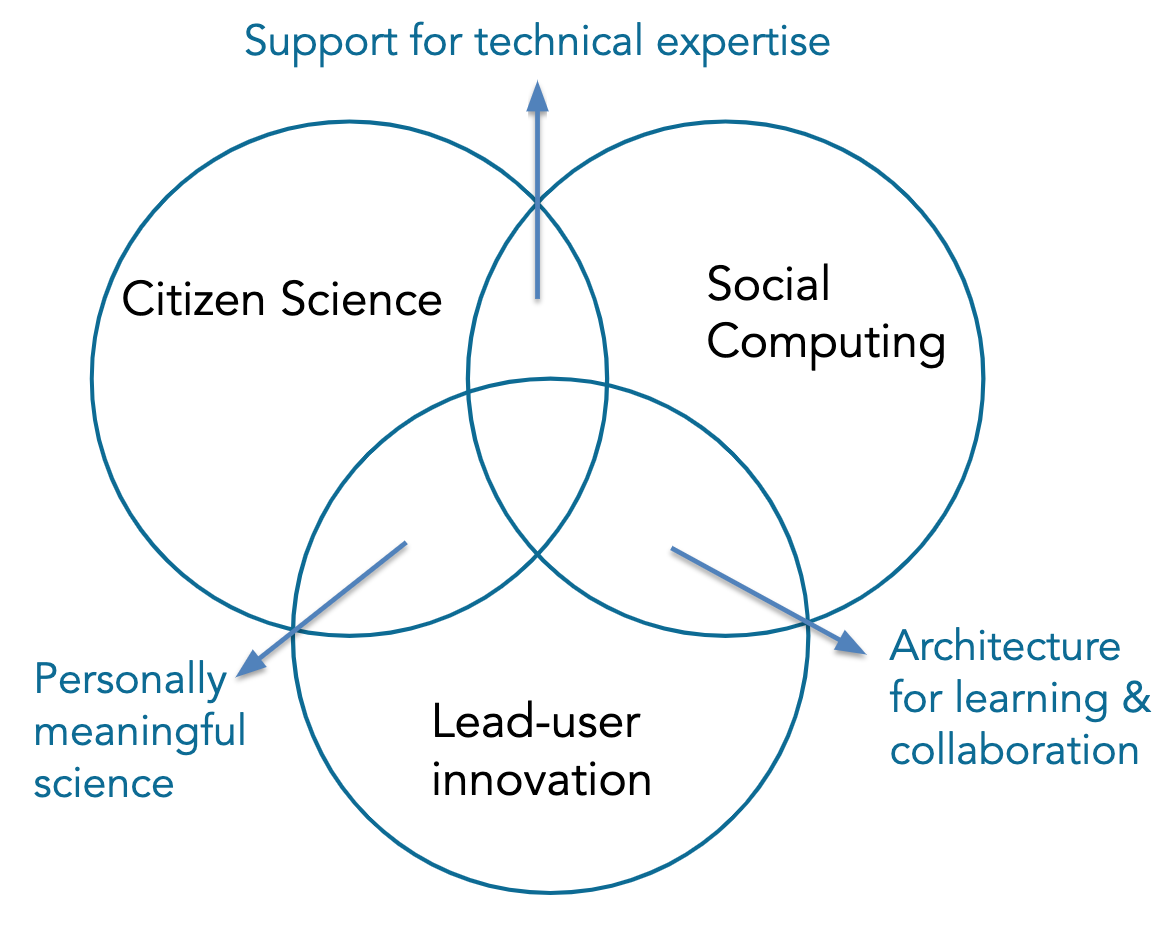
\includegraphics[width=0.4\textwidth]{figures/2-related/venn.png}
  \caption[]
{This dissertation draws from and contributes to citizen science, lead-user innovation, and social computing\index{related-1}}
  \label{fig:related-1}
\end{figure}

\vspace{0.25in}

%So, we find that there are three main challenges for citizen science: 1) make it personally meaningful, 2) deepen the contributions that citizens can make. 3. 1. Improve the quality of poor contributions — and improve the quality of max contributions     1. — hockey stick curve 
%%%%%%
\section{Science is increasingly networked but misses people’s lived experience }
Science is increasingly networked, multidisciplinary, and
open~\cite{Pandey2017}. For instance, LIGO’s pathbreaking discovery of
gravitational waves brought together over 100 researchers
from over 100 institutions across 18 countries (ligo.org/about). 
Scientists increasingly share data and results faster (arxiv.org). 
Large scientific projects, like the Human Genome Project, 
took to agile science by sharing methods, data, and insights to 
collaboratively speed discoveries. Scientists also form global 
collaborations to accelerate research in nascent scientific domains, 
like the Earth Microbiome project (earthmicrobiome.org).
At its best, institutional science has benefitted immensely
from large-scale global collaboration. Complementing this success,
many online projects enable people to help scientists~\cite{Nielsen2012}: annotating 
scientific papers~\cite{Good2013}; labeling galaxies~\cite{JordanRaddick2013}; and providing microbiome 
samples~\cite{McDonald2018}, CPU cycles (worldcommunitygrid.org), or personal data (openhumans.org). 
Efforts to further expand participation in scientific research are bearing fruit: Lab in the Wild 
recruits anyone with an internet connection for behavioral studies~\cite{Reinecke2015}; and All of Us aims 
to recruit one million Americans from all strata of society (allofus.nih.gov). Such collaborative efforts from experts 
and citizens suggest a new model for scientific work.

Often, when citizens participate in science, it is as “embedded sensors” that 
are aggregated by experts. Public involvement in scientific endeavors continues
to be largely limited to performing tasks just beyond the reach of computers.
A classic example is Audubon’s Christmas bird count, run since 1900
~\cite{Audubon2016}. Online examples include reporting flower blooms in
Project Budburst~\cite{BoulderColorado2016}; recording wildlife activity~\cite{Faridani2009a};
identifying galaxies from satellite imagery in GalaxyZoo~\cite{Zooniverse2007}; 
and biochemistry games: finding protein structures in Foldit~\cite{Cooper2010}, 
synthesizing RNA molecules in EteRNA~\cite{Lee2014}, and aligning 
nucleotide sequences in Phylo~\cite{Kawrykow2012}. Distributed 
data contributions from people around the world—browsing online~\cite{Coviello2014}, using activity trackers, and joining scientific projects—have enabled valuable insights on topics including 
obesity~\cite{Althoff2017}, aesthetic preferences~\cite{Reinecke2014a}, sleep~\cite{F.lux2019}, and the human microbiome~\cite{McDonald2018a}. At their
best, these citizen science platforms yield novel insights.
For example, Foldit players discovered protein structures
that helped scientists understand how the AIDS virus reproduces~\cite{Coren2011}. Why have such collaborative efforts succeeded?


%Different people provide different expertise that can vet claims and  fix mistakes~\cite{kane2009s}.
Collaboration benefits creativity when it brings different
 perspectives that build on each other; it impedes creativity (or worse, causes regression) 
when—through groupthink—it spreads biases rather than removing them~\cite{starbird2014rumors}. 
A humbling example of the power of fresh eyes: volunteer citizen scientists identified a new class of 
galaxies (“green pea” galaxies) after researching green blots on Galaxy zoo images; 
experts had dismissed these images as apparatus error~\cite{cardamone2009galaxy}.
This volunteer-led discovery demonstrates the need for fostering independent perspectives 
while simultaneously cultivating sufficient knowledge for meaningful domain contributions. 
Such collaboration requires strategic isolation: roviding just enough scaffolding to keep 
biases independent, while not stifling original ideas for bottom-up knowledge creation.

%This dissertation draws on the idea of people using  cognitive surplus to collaboratively answer scientific questions~\cite{Bonney2009}.


%%%% - where does this go
%Such bite-sized contributions is not without reason—a lot of
%scientific work requires deep conceptual knowledge and 
%training in scientific process to perform useful work. Most
%citizens lack the time, resources, and motivation to develop
%narrow, unique skillsets. Expanding the depth and breadth of work 
%performed by citizen science communities would be useful.

%\subsection{Citizen Scientists: From Collectors to Experimenters}
\subsection{Opportunity: Can people be scientists rather than just sensors?}
Citizens have successfully solved expert-defined problems as sensors or algorithms with a 
row-filling model of contribution.
In the quest to get people to track, measure, accumulate, or
sort both digital and analog data, citizen science has overlooked the massive 
opportunity of leveraging people’s unique advantages: our skills as reflective, 
creative thinkers who generate theories about the world, including ourselves.
People can offer more than just their data and perceptual
skills: they create theories, right or wrong, about a wide
range of topics including emotions~\cite{Johnson-Laird1992a}, motivation~\cite{Markus1991}, or
diet. These may be observational theories~\cite{Kempton1986}, folk theories
passed in a family/culture across generations~\cite{Gelman2011}, or ideas
brainstormed in online communities~\cite{23andme2016}. Perhaps, these intuitions 
can provide a starting point for independent, participatory experience that also assists the scientific community.

When are such personal experiences worth paying attention
to? For every intuition proven right, many more may be
closer to snake oil — e.g., the widespread belief in the utility
of probiotics despite limited evidence~\cite{Bonifait2009}. The global internet
increases the proliferation of both powerful and questionable
ideas: sharing speculation is fast while evaluation remains
slow. Moreover, people develop intuitions of cause and effect
that may or may not be correct. Current online forum
designs prioritize discussion — sharing personal details in
long, free-flowing text — over structure, succinctness, learning,
and potential scientific utility~\cite{Thomas2002}.

Advances in precision medicine have demonstrated the need
to engage people in uncovering and sharing insights~\cite{Aronson2015}. People
are highly motivated to improve their health outcomes,
more so if they suffer from a condition that severely affects
their quality of life, naturally forming communities. For example,
patients from the Amyotrophic Lateral Sclerosis
(ALS) community on Patients Like Me (patientslikeme.com)
organized a study to track effects of Lithium on their symptoms
~\cite{Wicks2011}. This is not surprising; lead users excel at tackling
need-intensive problems where they can use their lived
experiences to identify problems, try solutions, and readily
observe the effects~\cite{VonHippel2005}. Other organized communities like
Quantified Self hope to uncover lifestyle patterns that may
improve their productivity and health outcomes. The word
‘self’ belies the fact that such movements are highly collaborative:
amateurs frequently share experiences and invite
feedback on online fora (patientslikeme.com) and blogs
(ibsgroup.org). Millions follow these ideas and some incorporate
these intuitions in their lives. What kinds of scaffolds
and structure may help people generate better ideas and implement them as actionable plans that
enable researchers to identify promising insights?

%How can people expand their insights into scientific work?

Most scientists develop their skills through an apprenticeship-
based graduate school experience. Apprenticeships emphasize
hands-on experience with individualized, taskspecific
feedback~\cite{schon1984reflective}. Scientists possess a wealth of declarative
knowledge about their domains (e.g., how to set up a
randomized controlled trial), and also procedural knowledge
—some narrow, some broad —towards getting things done
(e.g., improving fMRI signal intensity by having participants
consume cocoa beforehand~\cite{Francis2006}). This dissertation explores how
online learning and process training systems, combined with
peer collaboration, can help people learn similar skills that
can be useful in scientific domains.
%So, we find that there are three main challenges for citizen science: 1) make it personally meaningful, 2) deepen the contributions that citizens can make. 3. 1. Improve the quality of poor contributions — and improve the quality of max contributions     1. — hockey stick curve 
%WOULDN'T IT BE GREAT TO HAVE PEOPLE DESIGN AND RUN EXPERIMENTS AS AN INSTANCE OF COMPLEX SCIENTIFIC WORK
%Link to lead users -- people already doing personally meaningful work.. 

%%%%%%%%%%%%%%%%%%
\section{Lead users Succeed When They Know What to Do and How to Do It}
%“Lead users are rarely experts by themselves. They are novices who find themselves at the right place, with the right tools (that they might have created themselves), and who have the courage to follow through.” Lead users have created different—and in some cases better designs— than experts. 

%examples: UN example (see eric vh)

Lead-user innovation is both an inspiration and an application area for this dissertation. Lead users are
users of a product (or service) who experience advanced needs unmet by existing products~\cite{VonHippel2005}. The
power of lead-user innovation is that lived experience, a tight feedback loop, and strong personal
motivation can yield different and sometimes better products than experts [32]. For example, diabetes
patients have improved insulin delivery [47] and snowboarders have improved their binding
ergonomics. Lead users also collaborate online to build software
(github.com), create novel hardware \& reference designs
(openaps.org), and share personal data (quantifiedself.com,
openhumans.org). Some go further still, e.g., the transcranial
direct-current stimulation community draws ideas from scientific
papers to attempt self-experiments (reddit.com/r/
tDCS). In a few exceptional cases, lead users have even authored
scientific papers, e.g., Open Artificial Pancreas creator
Dana Lewis discussed the benefits and challenges of first-generation
automated insulin delivery at the 2016 American
Diabetes Conference~\cite{DanaLewis}.

Why do people do this? Curiosity, personal learning, and social
comparison are three reasons~\cite{Reinecke2015}. A massive interest in
personal genomics (over 1 million 23andme participants)
and, more recently, the human microbiome (13,000 American
Gut Project participants, americangut.org) demonstrate
people’s urge to understand what makes them who they are.
Users of these platforms send data, answer survey questions,
and discuss on fora. Some even use online lectures to understand
concepts of genes, phenotypes, and microbiota they
may not have perused otherwise~\cite{23andMe2017, Knight2016}. 

\subsection{Opportunity: Providing lead users the expertise to tackle complex knowledge work}
Lead users have an advantage when the key ingredient is experience intensive; experts retain the
advantage for solution-intensive innovations [32].  Sometimes, having a different background
 than experts can be beneficial. Shared knowledge is great when it’s right, but blocks progress
 when wrong. When false assumptions limit experts, at least some novices are likely to be 
“uninfected”. The converse also holds, and much more often: novices are also “uninfected” 
by all the knowledge that enables experts to innovate. In a large distributed community, 
there’s often someone who happens to have important relevant knowledge, usually 
drawing on a relevant but distant domain. Having many people work on the same problem 
increases the odds that one will break through. Drawing on secondary expertise as 
inspiration can be an important agent of creativity because almost by definition, the
 combination is rare~\cite{Boden2004}. 
%For example, GalaxyZoo volunteers discovered ‘green pea’ galaxies overlooked by scientists who mistakenly assumed the green hue was merely an imaging artifact~\cite{Tinati2015}. 

Community-driven approaches to understand personal
health and well-being largely reside outside the realm
of institutional science and medicine. While some fads and beliefs are 
questionable at best, on occasion communities
break new ground that may provide widespread value,
such as fecal transplants to alleviate Clostridium difficile infection
symptoms~\cite{Brandt2012}. Some doctors recommend that patients
track their symptoms and reflect upon them to find
insights. Putting people in charge can help them find significant
relief for ailments like chronic migraine~\cite{Gawande2017} and provide
researchers and clinicians with useful patient data
(smartpatients.com). Insights from N = 1 studies have helped
crack scientific puzzles about the working of the mind~\cite{V.S.Ramachandran1998},
heart, and microbes~\cite{Weisse2012}. 

Personal needs and challenges can be highly motivating but performing complex work still requires multiple rounds of trial and error. 
People need to know the genre of work and implement it correctly.  Professionals have the advantages of training, conceptual knowledge, 
pre-existing organizational structure for 
collaboration and support, and direct access to resources. Lead users either seek these resources from others or need to create them. 
Providing a correct and complete model for complex, structured activities might reduce efforts and improve the quality of results.
This dissertation reduces the gap between lead users' ideas and implementation by providing templates for 
genre work using just-in-time training and a collaboration platform to find others. This dissertation focuses on enabling people transform their idea to a controlled experiment as opposed to 
self-tracking or informal iteration which is the focus of most current citizen-led work in health.

\subsection {Case: Scientific experimentation is difficult}
While public contributions have supported institutional science; it’s rare for citizens to design
their own experiments. A number of health and behavioral research projects enlist citizens as helpers (e.g., HabitLab [43]). 
CivilServant enables online communities’ 
moderators to test policy ideas; moderators share these ideas with researchers who transform 
them to study designs [51]. Through the PatientsLikeMe website (patientslikeme.com), citizens 
and scientists created a study investigating whether consuming lithium alleviated ALS symptoms [64]. 
While an initial scientific study had provided positive benefits, both this citizen science study and 
a subsequent university study did not find benefits. Tummy Trials asked 
participants to generate health questions, introducing a protocol for self-experimentation 
combining ideation and self-tracking [36]. In all these cases, citizens rely on experts to provide sound experimental design.

Why is experimentation hard?  Despite a predetermined goal and a formalized process, experimentation
requires making situationally-appropriate decisions. A dependent variable may produce crisp
numbers but feedback on the experiment design itself is more multifarious. Good experiment
design is inherently user centered: how will participants interpret the instructions? Experiment
designers need awareness of others’ interpretation of their ideas and asks. Feedback and iteration
might be key to creative success, especially for novices. Providing feedback on experiment
designs requires knowing the success criteria and how to
help improve.  Feedback can be provided by experts~\cite{dow2012shepherding, schon1984reflective}, peers~\cite{Boud1995, Kulkarni2015b}, software~\cite{Dantoni2015, Head2017}, or even oneself~\cite{Boud1995,schon1984reflective}. While feedback from novices can
potentially improve both structure and content, it can also emphasize superficial issues over the
underlying structure~\cite{chi1981expertise}. Finally, successfully running an experiment
requires managing multiple processes such as random
assignment, anonymizing participant details, and sending
instructions and reminders for data collection.

%%%%%%%%%%%%%%%%%%%%%%%%%%%%%%%%%%%%%%%%%%%%%%%%%%%%%%%%%%%%%%%%%%%%
%But to understand that let's look at social computing ideas...

\section{Social Computing and Crowdsourcing Architectures for Complex Work}
Canonical crowdsourcing breaks larger tasks into microtasks; algorithms specify the division,
dependency, and agglomeration activities while workers perform small tasks supported by task-specific
guidelines~\cite{kittur2012future}. Leveraging existing expertise is one approach for complex knowledge work. One strategy
directly employs experts’ just-in-time feedback to improve crowd work~\cite{dow2012shepherding}. Workflows manage
experts for open-ended work like developing interactive prototypes~\cite{Retelny2014}. 
Flash Organizations uses automated hiring, a hierarchy with a central leader, and optional 
team leaders for collaborative projects like product design~\cite{Valentine2017}.
Another strategy creates roles that enable more experienced crowd members to orchestrate
the work. Ensemble supports leaders in guiding and constraining crowd 
contributions~\cite{Kim2014e}. Role-based approaches confer three benefits: 1) clean 
delineation of responsibilities improves chances of task completion, 2) clustering similar tasks 
reduces overhead and increases consistency; 3) people can decide their contribution levels. 
However, experts are expensive, in short supply, and sometimes prone to groupthink. 

Carefully-constructed interfaces can aid novices with task-specific expertise to solve problems 
that only experts previously could. Foldit introduced 3D game for specifying low-energy protein 
structures via direct manipulation~\cite{Cooper2010}. Making a challenge visually salient is an 
effective way to on-board novices. For tasks that don’t have as a crisp visual analogue as protein
folding, people need better conceptual support. For more abstract tasks, CrowdLayout and Cicero
provide guidelines and static rules that crowdworkers can use to reason about their choices and
to improve layouts of biological networks~\cite{Singh:2018:CCD:3173574.3173806, chen2019cicero}.
This dissertation explores scaffolds that are more structural than visual.

Prior work has explored  collaborative hypothesis generation and testing on pre-existing data sets
~\cite{luther2009pathfinder,willett2011commentspace}. This dissertation offers a 
complementary contribution: enabling citizens to generate data on topics of personal interest. 

One way to make complex tasks manageable is to divide them into distinct phases. 
Touchstone demonstrates the power of a semi-automated workflow integrating experiment 
design, testing, and analysis~\cite{Mackay2007}. Crowdsourcing has similarly innovated by 
creating distinct phases: break larger tasks into microtasks; algorithms specify the division, 
dependency, and agglomeration activities while workers perform small tasks supported by 
task-specific guidelines~\cite{lasecki2012real}. From these systems, our work draws the 
idea of dividing experimentation into multiple tasks—some self-sourced, others 
crowd-sourced; and introduce just-in-time domain expertise to perform these tasks. 

 
%How might groups of novices perform complex work like experimentation?
%Systems like Foldit and EteRNA powerfully show  how carefully-constructed interfaces provide
%novices with the task-specific expertise to solve problems that only experts previously 
%could~\cite{Cooper2010, Lasecki2012, Lee2014, Zooniverse2007}.

%%%%%%%
%%building up solution space - more work
\subsection{Learning resources at the right time}
Providing just-in-time supports, step-by-step instruction, and showing helpful supportive
 information are core ideas in instructional design~\cite{Kirschner2008}. Crowdsourcing 
systems leverage interactive guidance for specific tasks. For example, CrowdLayout and 
Cicero provide guidelines and static rules that workers use these to reason about their choices
 and improve network layouts~\cite{chen2019cicero, Singh:2018:CCD:3173574.3173806}. 
Others like CrowdSCIM and Crowdclass scaffold pre-task interventions~\cite{Lee2016,wang2018exploring}. 
While learning resources are distributed across the internet, they are rarely integrated with the task. 

Creative, open-ended work has rich pedagogical value. Online work, like 
online learning, requires appropriate scaffoldings, such as rubrics
~\cite{Boud1995, Kulkarni2013peer}, decision trees~\cite{Lee2016,Yu2006}, 
tutorials~\cite{Andersen2012}, and quick expert guidance~\cite{dow2012shepherding}. 
Similar to general critique of pure discovery learning~\cite{Mayer2004}, simply 
asking participants to “figure it out” would be poor pedagogy. Hence, this dissertation
introduces a guided discovery learning approach as Mayer advocates: expert-curated 
learning materials help participants start, with discovery following. Such integration 
offers a Problem-based learning experience with context and 
motivation for the material students learn~\cite{Savery1995}. In principle, these 
real-world problems also provide a yardstick for measuring learning. 

This dissertation introduces support during the task itself for those with little-to-no mental model of the knowledge domain. 
Like the Shepherd review-writing system~\cite{dow2012shepherding}, this dissertation provides just-in-time support. 
There are two key differences: 1) this work scaffolds the entire creation process, not just the post-draft feedback
 stage, and 2) it does not draw on expert time – the knowledge is implemented in the software itself. 
%todo-repeated too many times


%%%%%%%%%%%
\section{Microbiome research: a petri dish for personally meaningful scientific work}
The human microbiome is the collection of all microbes and
their genetic components in and on our bodies. It is highly
personal: each of us hosts a different collection of microbes,
and this collection is influenced by our environment, diet,
health, lifestyle, and genetics. A major scientific effort is to
better characterize and understand this diversity and the
causal factors for it (hmpdacc.org). Understanding the human microbiome requires insights
into people’s lifestyles. Microbiome science is nascent, highly contextual, and personally motivating.
However, research has only scratched the surface of understanding the microbiome and using it 
to improve our wellbeing. Engaging diverse participants at scale can potentially yield exciting new results.


The American Gut Project (americangut.org) offers a
crowdsourced opportunity for people to get a microbiome
sampling kit~\cite{KnightLab2016a}. AGP
participants contribute their samples for bacterial marker
gene sequencing and analysis~\cite{Debelius2016}. Participants then receive
a summary of their results with all their raw data. Anonymized data is publically available.

To date, more than 13,000 people have participated.
Participants submit both a physical sample and fill out
a survey. AGP seeks to build a comprehensive map of the human microbiome, and identify
its healthy and unhealthy components. Analysis has revealed lifestyle-microbiome correlations
of dog ownership and beer or vegetable consumption,
among others.

\subsubsection{People hold the key to understanding the gut microbiome}
The structure of the human microbiome is influenced by many factors, including age, genetics, diet, and xenobiotic and antibiotic use~\cite{Gill2006}. The gut microbiome in particular plays an important role in metabolism and immune system development, and some microbiome dysbioses have been associated with diseases such as obesity, inflammatory bowel disease, type I and type II diabetes, autism, multiple sclerosis, and malnutrition~\cite{Cho2012}. The human microbiome is impossible to understand without information about its host~\cite{Debelius2016} and many influence factors remain unknown. Teaching people about the gut microbiome and having them guess associations between the microbiome and health and disease states can potentially accelerate the process of discovering links between diet, disease, and lifestyle factors and the gut microbiome.

Currently, the topics for scientific investigation are handpicked
by a small group of scientists. Can opening up the
scientific process to the world yield additional insights?
How can people’s situated knowledge supplement institutional
science? This dissertation provides systems and rechniques for novices to complement experts in creating new knowledge about the microbiome. \\

%Crowd workers perform better when they understand their efforts’ importance. For example, Mechanical Turk workers analyzing radiology images performed better when told of the medical purpose: finding cancerous tumors~\cite{Chandler2013}. Motivation can also be personal. For example, 23andMe is a genetic testing site and online service that includes a discussion board. On this forum, a user reported disliking the sounds of others eating. She’s not alone; a 23andMe survey found 16,000 users with the same condition and a predictive genetic similarity among them~\cite{23andMe2016}.

This chapter provided an overview of related research; chapters dedicated to specific systems discuss additional research that informs that design of those systems. This dissertation explores integrating learning in social computing for complex, creative work with two goals in mind: efficacy of the resulting systems (i.e. usability, correctness, and existential evidence) and generality of the underlying techniques upon which the tools are built.